\documentclass{article}

% ---------------------------------------------------------------
% Final report. Uses the Overleaf "arXiv & Prime AI style" template (arxiv.sty).
% A compatible arxiv.sty is included so the file also compiles offline.
% Every number in the tables is generated by experiments/make_tables.py from results/*.json.
% ---------------------------------------------------------------
\usepackage{amsmath,amssymb,amsthm}
\usepackage{arxiv}
\usepackage[utf8]{inputenc}
\usepackage[T1]{fontenc}
\usepackage{hyperref}
\usepackage{url}
\usepackage{booktabs}
\usepackage{amsfonts}
\usepackage{nicefrac}
\usepackage{microtype}
\usepackage{graphicx}
\usepackage{natbib}
\usepackage{tabularx}
\usepackage{enumitem}
\usepackage{xcolor}
\usepackage{algorithm}
\usepackage{algpseudocode}
\usepackage[font=small,labelfont=bf,skip=3pt]{caption}

\newtheorem{definition}{Definition}
\newtheorem{proposition}{Proposition}

\newcommand{\E}{\mathbb{E}}
\newcommand{\1}{\mathbb{1}}
\newcommand{\N}{\mathcal{N}}
\newcommand{\crore}{\text{\,cr}}
\newcommand{\rupee}{\text{Rs.\,}}
% >>> Replace with your public repository URL before submitting <<<
\newcommand{\repourl}{https://github.com/harshmasalge/BIDDING-UNDER-UNCERTAINTY-AND-BUDGETS-A-MULTI-AGENT-STUDY-OF-THE-IPL-PLAYER-AUCTION}

\setlist{leftmargin=*,itemsep=1pt,topsep=2pt}
\setlength{\textfloatsep}{8pt}
\setlength{\floatsep}{6pt}

\title{Bidding Under Uncertainty and Budgets:\\ A Multi-Agent Study of the IPL Player Auction}
\date{}
\author{
  Harshvarshan Masalge \\ 24110196
  \And
  Advait Andhale \\ 24110039
  \And
  Onkar Gaikwad \\ 24110117
  \And
  Shreyash Pandit \\ 24110334
}
\renewcommand{\headeright}{Final Report}
\renewcommand{\undertitle}{CS329 Foundations of AI: Multiagent Systems -- Project Implementation \& Report}
\renewcommand{\shorttitle}{Bidding Under Uncertainty and Budgets}
\hypersetup{pdftitle={Bidding Under Uncertainty and Budgets: A Multi-Agent Study of the IPL Player Auction},
  pdfauthor={Masalge, Andhale, Gaikwad, Pandit}, colorlinks=true, linkcolor=blue!50!black, citecolor=blue!50!black, urlcolor=blue!50!black}

\begin{document}
\maketitle

\begin{abstract}
We model the Indian Premier League (IPL) player auction as a sequential, budget-constrained, common-value auction among ten teams and study it with a simulator built on real data: Cricsheet ball-by-ball records (1{,}243 matches), auction outcomes for 2018--2025, and the full 577-player list, purses and retentions of the 2025 mega auction. Player values come from an empirical-Bayes performance model whose money scale is fitted on the \emph{2022} auction and tested out-of-sample on 2025 ($R^2=0.53$ on log price, Spearman $0.76$). We find that (i) the winner's curse is large when purses are slack (naive winners pay $1.23\times$ true value) but is \emph{masked} by binding purses: prices fall to $0.83\times$ value while the winners' estimates remain biased upward; (ii) budget-aware bidding by dynamic programming, using a closed-form drop-out rule that we prove and verify numerically, earns $1.6$--$4.4\times$ the utility of myopic bidding, with the largest gains when purses are tight; (iii) best-response dynamics over pacing multipliers cycle rather than converge, although their time-average is an approximate equilibrium whose simulated prices match the real 2025 price distribution better than naive bidding (KS $0.13$ vs.\ $0.23$); (iv) agents that learn without an opponent model (dual pacing, Q-learning) recover at most $29\%$ of the DP's gain; and (v) making values team-specific through each team's best playing XI changes a player's worth by a factor of about $3.5$ across teams and improves both team outcomes and the fit to real allocations.
\end{abstract}

\keywords{Sequential auctions \and Winner's curse \and Budget pacing \and Constrained MDP \and Multi-agent learning}

% ===============================================================
\section{Introduction}
\label{sec:intro}
In the 2025 IPL mega auction, ten franchises spent \rupee639\crore{} on 182 of 577 listed players~\citep{kaggle_auction}. Each franchise bids live against the others, on players whose future value is uncertain, from a fixed purse that must also complete a squad of 18--25 players with at most 8 from overseas. This combines three classic difficulties: strategic interaction, common values with noisy estimates, which produce the \emph{winner's curse}~\citep{capen1971,wilson1977,milgrom1982,thaler1988}, and a budget that couples every decision in the auction~\citep{benoit2001}. The same structure underlies budget pacing in online advertising~\citep{borgs2007,balseiro2019,conitzer2022}.

The idea review posed this as a Bayesian game with a constrained-MDP view of each team's budget and four research questions (Section~\ref{sec:rq}). This report answers them and addresses the three review comments:
\begin{enumerate}
  \item \textbf{Independent validation.} The money scale is now fitted on the 2022 auction (and, as a robustness check, on 2018--2024) and tested on 2025. Opponent behaviour for the validation is computed inside the simulator, not tuned on 2025 outcomes (Sections~\ref{sec:m-data},~\ref{sec:r-valid}).
  \item \textbf{Team-specific values.} Utilities can be the value of each team's \emph{best playing XI} given its retained players and purchases, solved exactly. Need-aware agents bid their own marginal value (Sections~\ref{sec:m-xi},~\ref{sec:r-xi}).
  \item \textbf{Tight budgets first.} The prototype's tight-budget behaviour was fixed and explained before any RQ was run: binding purses cap prices, which hides the winner's curse in the overpayment metric while the belief bias remains (Sections~\ref{sec:m-sim},~\ref{sec:r-curse}).
\end{enumerate}

% ===============================================================
\section{Preliminaries}
\label{sec:prelim}
$\N=\{1,\dots,n\}$ is the set of teams ($n=10$); lots (players) $j\in\{1,\dots,K\}$, $K=577$, are sold in order $\pi$. Lot $j$ has reserve (base) price $r_j$, overseas flag $o_j$ and role $g_j\in\{\textsc{bat},\textsc{wk},\textsc{ar},\textsc{bowl}\}$. Before lot $j$ team $i$ has purse $b_{ij}$, squad size $m_{ij}$ and overseas count $q_{ij}$, starting from $(B_i,m_i^0,q_i^0)$ after retentions. The rules require
\begin{equation}
 \underline m\le m_i^{\rm final}\le \overline m,\qquad q_i^{\rm final}\le\overline q,\qquad(\underline m,\overline m,\overline q)=(18,25,8).\label{eq:squad}
\end{equation}
\begin{definition}[Common value, private signals]
$\log v_j\sim\mathcal N(\mu_j,s_j^2)$ is common to all teams; team $i$ observes $x_{ij}=\log v_j+\varepsilon_{ij}$, $\varepsilon_{ij}\stackrel{\rm iid}{\sim}\mathcal N(0,\sigma^2)$. The naive estimate is $\hat v_{ij}=\E[v_j\mid x_{ij}]=\exp(\bar m+\bar s^2/2)$ with $\bar m=\omega x_{ij}+(1-\omega)\mu_j$, $\bar s^2=\omega\sigma^2$, $\omega=s_j^2/(s_j^2+\sigma^2)$.
\end{definition}
\begin{definition}[Winner's curse]
With winner $w_j$ and price $p_j$: the \emph{overpayment} $\E[p_j-v_j]$ and the \emph{belief bias} $\E[\hat v_{w_jj}-v_j]$ over sold lots.
\end{definition}
The ascending auction is modelled by drop-out prices (``button'' model~\citep{krishna2009}). An MDP $(\mathcal S,\mathcal A,P,R,T)$ is solved by backward induction~\citep{puterman1994}; a constrained MDP restricts a cumulative cost~\citep{altman1999}. A bidder \emph{paces} with $\lambda\ge0$ if it bids $\hat v/(\alpha+\lambda)$, and a profile $(\lambda_i)$ is a pacing equilibrium if no team gains by changing its own multiplier~\citep{conitzer2022}.

% ===============================================================
\section{Problem Formulation}
\label{sec:formulation}
\paragraph{Mechanism.} Team $i$ may bid on lot $j$ only if $m_{ij}<\overline m$, $o_j=0\vee q_{ij}<\overline q$, and its cap
\begin{equation}
 \bar a_{ij}=b_{ij}-\underline r\,(\underline m-m_{ij}-1)^+,\qquad \underline r=0.30\crore,\label{eq:cap}
\end{equation}
is at least $r_j$. With drop-outs $a_{ij}\le\bar a_{ij}$ and the two highest $a_{(1)}\ge a_{(2)}$, the lot is unsold if $a_{(1)}<r_j$, otherwise
\begin{equation}
 w_j=\arg\max_i a_{ij},\qquad p_j=\max\{r_j,\ \min(a_{(1)},a_{(2)}+\delta)\},\qquad\delta=0.05\crore.\label{eq:mech}
\end{equation}
\paragraph{Utility.} $U_i=f_i(S_i)-\alpha\sum_{j\in S_i}p_j$, with $\alpha=1$ (quasi-linear) in all experiments. In the \emph{common-value} model $f_i(S)=\sum_{j\in S}v_j$. In the \emph{team-specific} model (feedback 2)
\begin{equation}
\begin{aligned}
 f_i(S)&=\mathrm{XI}_i(S)+\eta\big(\textstyle\sum_{k\in R_i\cup S}v_k-\mathrm{XI}_i(S)\big),\\
 \mathrm{XI}_i(S)&=\max_{X\subseteq R_i\cup S,\,|X|=11}\Big\{\textstyle\sum_{k\in X}v_k:\ \sum_X o_k\le4,\ \#\textsc{wk}\ge1,\ \#(\textsc{bowl}\cup\textsc{ar})\ge5,\ \#(\textsc{bat}\cup\textsc{wk})\ge4\Big\},
\end{aligned}\label{eq:xi}
\end{equation}
where $R_i$ are team $i$'s retained players and $\eta=0.2$ values bench cover. A player's marginal worth $f_i(S\cup\{j\})-f_i(S)$ now depends on the team and on its current squad.

\paragraph{Equilibrium bid.} Ignoring budgets, the symmetric equilibrium of the second-price common-value auction bids the value conditional on tying with the strongest rival~\citep{milgrom1982,krishna2009}:
\begin{equation}
 \beta(x)=\E[v\mid x_1=x,\ \max_{k\ne1}x_k=x]=\frac{\int e^u\,\phi(x;u,\sigma^2)^2\,\Phi(x;u,\sigma^2)^{n-2}\,\phi(u;\mu,s^2)\,du}{\int \phi(x;u,\sigma^2)^2\,\Phi(x;u,\sigma^2)^{n-2}\,\phi(u;\mu,s^2)\,du}.\label{eq:beta}
\end{equation}
\paragraph{Budget allocation as a constrained MDP.} For a focal team, let $D_t$ be the highest rival drop-out on the $t$-th lot $j=\pi(t)$, with joint law $G_t$ of $(v_j,D_t)$. With $p=\max(r_j,D_t+\delta)$, state $(b,m)$ and value-to-go $V_t$,
\begin{equation}
 V_t(b,m)=\E\Big[\max_{a\le\bar a}\big\{\1\{a\ge p\}\big(v_j-\alpha p+V_{t+1}(b-p,m{+}1)\big)+\1\{a<p\}V_{t+1}(b,m)\big\}\Big],\label{eq:bellman}
\end{equation}
with $V_{K+1}(b,m)=\alpha(b-\underline r k)+k\,\bar v_{\rm fill}$ for the $k=(\underline m-m)^+$ mandatory fills ($-\infty$ if unaffordable).
\begin{proposition}[Indifference drop-out]\label{prop:threshold}
If $V_{t+1}(\cdot,m+1)$ is non-decreasing in $b$ and the team evaluates the lot by $\hat v$ independently of $D_t$, the optimal drop-out does not depend on $G_t$:
\begin{equation}
 a_t^\ast=\min\Big\{\bar a,\ \sup\{p\ge r_j:\ \hat v-\alpha p\ \ge\ V_{t+1}(b,m)-V_{t+1}(b-p,m{+}1)\}\Big\}.\label{eq:threshold}
\end{equation}
\end{proposition}
\begin{proof}
Since the price is $p(D_t)$ and not $a$, dropping out at $a$ yields $h(p)+V_{t+1}(b,m)$ if $a\ge p$ and $V_{t+1}(b,m)$ otherwise, where $h(p)=\hat v-\alpha p+V_{t+1}(b-p,m{+}1)-V_{t+1}(b,m)$. For every realisation of $D_t$ the best outcome is to win exactly when $h(p)\ge0$ (and $p\le\bar a$). Because $\alpha\ge0$ and $V_{t+1}(\cdot,m{+}1)$ is non-decreasing, $h$ is non-increasing in $p$, so $\{p\ge r_j:h(p)\ge0\}$ is an interval $[r_j,a^\ast]$. Dropping out at $a^\ast_t$ (capped at $\bar a$) wins exactly on this interval, so it is optimal pointwise in $D_t$ and therefore for every $G_t$.
\end{proof}
Linearising $V_{t+1}(b,m)-V_{t+1}(b-p,m{+}1)\approx\lambda_tp+\omega_t$ gives $a^\ast_t\approx(\hat v-\omega_t)/(\alpha+\lambda_t)$: multiplicative pacing~\citep{balseiro2019} is a first-order approximation of~\eqref{eq:threshold}. Without an opponent model, a team can learn $\lambda$ online by projected dual sub-gradient descent~\citep{balseiro2019},
\begin{equation}
 \lambda_{t+1}=\Pi_{[0,\bar\lambda]}\big(\lambda_t-\eta(\rho-p_t\1\{w_t=i\})\big),\qquad\rho=B_i/K.\label{eq:dual}
\end{equation}
\paragraph{Benchmark.} With realised prices $\tilde p_j$ ($\tilde p_j=r_j$ if unsold), the hindsight-optimal squad solves
\begin{equation}
 \mathrm{OPT}_i=\max_{z\in\{0,1\}^K}\textstyle\sum_j(v_j-\alpha\tilde p_j)z_j\ \ \text{s.t.}\ \sum_j\tilde p_jz_j\le B_i,\ \ \underline m-m_i^0\le\sum_jz_j\le\overline m-m_i^0,\ \ \sum_jo_jz_j\le\overline q-q_i^0.\label{eq:ilp}
\end{equation}
\paragraph{Research questions.}\label{sec:rq}
\textbf{RQ1}: size of the winner's curse vs.\ $\sigma$, $n$ and purse tightness, and how much~\eqref{eq:beta} removes. \textbf{RQ2}: gain of budget-aware bidding (DP~\eqref{eq:bellman}--\eqref{eq:threshold}, pacing) over myopic bidding. \textbf{RQ3}: do best-response dynamics over pacing multipliers converge? \textbf{RQ4}: what is lost when the opponent model must be learned (\eqref{eq:dual}, Q-learning)?

% ===============================================================
\section{Methodology}
\label{sec:method}

\subsection{Data and value model (feedback 1)}\label{sec:m-data}
\paragraph{Data.} We parse 295{,}557 deliveries from 1{,}243 Cricsheet IPL matches (2008--2026)~\citep{cricsheet}, sold-player lists for 2018--2024, and the 2025 list (577 lots with base price, capped status, buyer and price)~\citep{kaggle_auction}. A separate ``enhanced'' Kaggle dataset turned out to contain synthetic player names and was discarded. Auction names are matched to Cricsheet names by surname and first initial, with a manual alias table and a rule that drops matches claimed by two different players. This matches 162 of the 182 players sold in 2025; 227 of the 577 lots have IPL data in the three pre-auction seasons. Purses and the 46 retained players are the public pre-auction state (Table~\ref{tab:teams}, Appendix).

\paragraph{Impact and empirical Bayes.} For every legal ball we compute a batting impact $z=$ runs $-$ season average $-W\cdot$(dismissal $-$ season rate) and a bowling impact $z=$ season runs-per-ball $-$ runs conceded $+W\cdot$(wicket $-$ season rate). Using only the three seasons before an auction (no look-ahead), the per-ball means are shrunk with the normal--normal model~\citep{efron1975}: $\hat\theta_j=w_j\bar z_j+(1-w_j)\mu$, $w_j=\tau^2/(\tau^2+\varsigma^2/n_j)$, $\mathrm{Var}(\theta_j\mid\bar z_j)=w_j\varsigma^2/n_j$, with $\varsigma^2$ the pooled within-player variance and $\tau^2$ estimated by the method of moments. The per-match impact is $I_j=\hat\theta^{\rm bat}_je^{\rm bat}_j+\hat\theta^{\rm bowl}_je^{\rm bowl}_j$, where $e$ is shrunk balls per match.

\paragraph{Money scale fitted on an earlier auction.} Following~\citet{karnik2010} we fit
\begin{equation}
 \log(p_j/P_y)=\gamma_0+\gamma_1I_j+\gamma_2\log(1+\text{matches}_j)+\gamma_3\1\{\text{record}\}+\gamma_4o_j+\gamma_{g_j}+e_j,\label{eq:hedonic}
\end{equation}
on the \textbf{2022 mega auction} (204 sold players), where $P_y$ is the per-team purse of year $y$, so the 2025 prediction is rescaled by $P_{2025}/P_{2022}=120/90$. The wicket value $W=15$ runs is chosen by leave-one-out error \emph{on 2022 only}. The 2025 prior is $\mu_j=\hat\gamma^\top X_j+\log P_{2025}$ and $s_j^2=s_0^2+\hat\gamma_1^2\mathrm{Var}(I_j)$, where $s_0=0.93$ is the residual spread net of impact uncertainty. Unknown nationality is imputed as overseas iff capped (every capped Indian in the list has an IPL record); unknown roles are drawn deterministically from the role mix of the known lots. Pooled 2018--2024 and in-sample 2025 fits are reported for comparison only.

\subsection{Simulator and the tight-budget fix (feedback 3)}\label{sec:m-sim}
The simulator runs the 577 real lots with the real purses and retentions. Lots are offered in set-wise order (capped before uncapped, higher base-price sets first, roles grouped, shuffled within a set); one fixed draw of this order is used for the DP experiments. The prototype behaved incorrectly with binding budgets for three reasons, each fixed before any RQ was run. (a) A ``stop shading near the end'' override made every strategy bid its full signal late in the auction. It is replaced by the real procedure: an \emph{accelerated round} in which teams take turns claiming unsold players at reserve when $\hat v-\alpha r_j>0$, followed by a mandatory fill at reserve for squads below 18. (b) Budgets were synthetic; they are now $(B_i,m^0_i,q^0_i)$ from 2025, and the cap~\eqref{eq:cap} reserves the real minimum base price for every mandatory slot. (c) Overpayment alone was reported. We now report both curse metrics plus the share of sales in which the winner's bid was \emph{cut by its cap}, which separates budget-masking from the curse itself. The ILP benchmark now uses realised prices~\eqref{eq:ilp} instead of a cost proxy. Unit tests check purse, squad and overseas invariants, the absence of a curse at $\sigma=0$, and its presence at $\sigma>0$ with slack purses.

\subsection{Team-specific values (feedback 2)}\label{sec:m-xi}
$\mathrm{XI}_i(S)$ in~\eqref{eq:xi} is solved \emph{exactly} by a dynamic program over count states (picked, overseas, wicket-keepers, bowling options, batters; $12\times5\times2\times6\times5$ states). It agrees with a MILP on 1{,}000 random squads and takes 0.4\,ms. A tracker keeps each team's DP table, so a marginal value costs one DP step. Retained players are valued with the same 2022-fitted scale. The \emph{need-aware} agent bids $[f_i(S\cup\{j\})-f_i(S)]/(\alpha+\lambda_i)$ using its own estimates.

\subsection{Agents}
\textbf{Naive} bids $\hat v$; \textbf{shade} bids $0.85\hat v$; \textbf{equilibrium} bids $\beta(x)$ from~\eqref{eq:beta} with $n$ the number of eligible teams (161-point quadrature); \textbf{pacing} bids $\hat v/(\alpha+\lambda)$; \textbf{dual pacing} follows~\eqref{eq:dual} with $\eta=0.02$, $\bar\lambda=3$. \textbf{DP} (Algorithm~\ref{alg:dp}) solves~\eqref{eq:bellman} on a \rupee0.25\crore{} purse grid using 40 pilot auctions to sample $(v_j,D_t)$ \emph{jointly}, so the value function prices in the winner's curse even though the decision uses $\hat v$; \textbf{DP+Eq.~(5)} uses $\beta(x)$ in place of $\hat v$ in~\eqref{eq:threshold}. \textbf{Q-learning}~\citep{watkins1992} learns a multiplier $\kappa\in\{0,.2,.35,.5,.75,1,1.25\}$ ($a=\kappa\hat v$) over states (auction quarter, purse per mandatory slot, squad need, $\hat v$ bucket) with reward $v_j-\alpha p_j$ on wins, $\epsilon$-greedy exploration decaying from 0.3 to 0.02, and no opponent model.

\begin{algorithm}[t]
\caption{Budget-aware DP bidder (full-information opponent model)}\label{alg:dp}
\small
\begin{algorithmic}[1]
\State Run $R=40$ pilot auctions against the opponent population; store $(v^{(r)}_j,D^{(r)}_t)$ for every lot.
\State $V_{K+1}(b,m)\gets\alpha(b-\underline r k)+k\bar v_{\rm fill}$ on the grid $b\in\{0,0.25,\dots,B_i\}$, $m\le25$.
\For{$t=K,\dots,1$} \Comment{vectorised over $(m,b,r)$}
  \State $p^{(r)}\gets\max(r_j,D_t^{(r)}+\delta)$;\ \ $x^{(r)}\gets\log v^{(r)}_j+\sigma\xi$;\ \ $\hat v^{(r)}\gets\E[v\mid x^{(r)}]$
  \State win$^{(r)}\gets$ feasible$(p^{(r)},b,m)\wedge\hat v^{(r)}-\alpha p^{(r)}+V_{t+1}(b-p^{(r)},m{+}1)\ge V_{t+1}(b,m)$
  \State $V_t(b,m)\gets\frac1R\sum_r\big[\text{win}^{(r)}(v^{(r)}_j-\alpha p^{(r)}+V_{t+1}(b-p^{(r)},m{+}1))+(1-\text{win}^{(r)})V_{t+1}(b,m)\big]$
\EndFor
\State \textbf{At lot $t$ live:} observe $x$; bid $a^\ast_t$ from~\eqref{eq:threshold} with $V_{t+1}$ (linear interpolation in $b$).
\end{algorithmic}
\end{algorithm}

\subsection{Pacing equilibrium and protocol}
For RQ3 every team paces. In each round of \emph{best-response (BR) dynamics} every team in turn picks $\lambda_i$ from a 10-point grid on $[0,6]$ to maximise its mean utility over 20 common-random-number seeds. We start from $\lambda\equiv0$ and $\lambda\equiv4$. Because plain BR cycles, we also run \emph{smoothed} BR (fictitious-play averaging~\citep{brown1951}, $\lambda_i\gets(1-\tfrac1k)\lambda_i+\tfrac1k\mathrm{BR}_i$) and measure each profile's $\epsilon$, the largest gain any team gets from a unilateral grid deviation. The lower-$\epsilon$ profile is used as $\lambda^\ast$: the realistic opponent population for RQ2, RQ4 and validation. Unless stated otherwise $\sigma=0.3$, $\alpha=1$, and results average 100 evaluation seeds disjoint from pilot and training seeds, with common random numbers across agents and 95\% intervals ($\pm1.96$\,s.e.).

% ===============================================================
\section{Results}
\label{sec:results}

\subsection{Out-of-sample money scale}\label{sec:r-scale}
\begin{table}[t]
\centering\small
\caption{Money scale~\eqref{eq:hedonic}: fitted on earlier auctions, evaluated on the 2025 auction (log price). MAE and bias in log units; the negative bias means 2025 prices were about 23\% below the purse-scaled prediction.}
\label{tab:scale}
\begin{tabular}{@{}lrrrrrr@{}}\toprule
& & train & \multicolumn{4}{c}{test: 2025 sold players ($n$=182)}\\\cmidrule(l){4-7}
Money scale & $n$ & $R^2$ & $R^2$ & Spearman & MAE & bias\\\midrule
Fit on 2022 (primary) & 204 & 0.57 & 0.53 & 0.76 & 0.72 & -0.27\\
Fit on 2018--2024 (pooled) & 704 & 0.41 & 0.54 & 0.77 & 0.75 & -0.29\\
Fit on 2025 (in-sample, old check) & 182 & 0.61 & 0.61 & 0.78 & 0.65 & +0.00\\
\bottomrule\end{tabular}

\end{table}
Table~\ref{tab:scale} answers feedback 1. Fitted on 2022 alone, the scale explains 53\% of the variance of 2025 log prices and ranks players with Spearman $0.76$. The non-independent in-sample check reported at the review overstated $R^2$ by about 0.08. Pooling 2018--2024 gives the same accuracy. The largest effects are overseas status ($\times2.9$) and IPL experience; impact adds $4.5\%$ per run/match. The remaining 0.93 log-unit residual becomes the common-value uncertainty $s_0$ of the auction model (Fig.~\ref{fig:scale}, Appendix).

\subsection{RQ1: the winner's curse, and why tight budgets hide it}\label{sec:r-curse}
\begin{figure}[t]
\centering
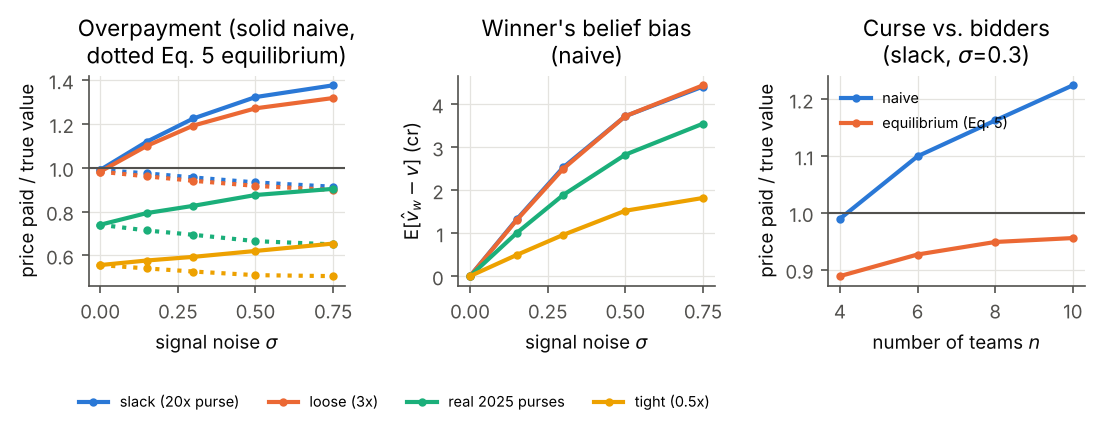
\includegraphics[width=0.9\linewidth]{../figures/fig_curse.png}
\caption{RQ1. Left: price paid relative to true value vs.\ signal noise for naive (solid) and Eq.~\eqref{eq:beta} bidders (dotted) under four purse regimes. Middle: belief bias of naive winners. Right: overpayment grows with the number of teams (slack purses). 100 seeds per point; error bars are smaller than the markers.}
\label{fig:curse}
\end{figure}
\begin{table}[t]
\centering\small
\caption{Winner's curse at $\sigma=0.3$ (all ten teams naive unless noted). $p/v$ = total price over total true value of lots sold in the auction; ``capped'' = share of sales where the winner's bid was cut by its purse cap~\eqref{eq:cap}.}
\label{tab:curse}
\begin{tabular}{@{}lrrrrrrr@{}}\toprule
& \multicolumn{5}{c}{naive bidders} & Eq.~(5) & \\\cmidrule(lr){2-6}\cmidrule(lr){7-7}
Purses & $p/v$, $\sigma$=0 & $p/v$ & $\E[p-v]$ & $\E[\hat v_w-v]$ & capped & $p/v$ & sold\\\midrule
slack ($20\times$) & 0.99 & 1.22 & +1.29 & 2.53 & 0.00 & 0.96 & 204\\
loose ($3\times$) & 0.98 & 1.19 & +1.13 & 2.50 & 0.03 & 0.94 & 190\\
real 2025 & 0.74 & 0.83 & -1.70 & 1.89 & 0.44 & 0.69 & 86\\
tight ($0.5\times$) & 0.56 & 0.59 & -3.70 & 0.96 & 0.61 & 0.53 & 60\\
\bottomrule\end{tabular}

\end{table}
With slack purses the curse appears as theory predicts (Fig.~\ref{fig:curse}, Table~\ref{tab:curse}). Naive winners pay $1.23\times$ the true value at $\sigma=0.3$ and $1.38\times$ at $\sigma=0.75$, and overpayment rises with the number of bidders from $0.99$ ($n=4$) to $1.23$ ($n=10$). The equilibrium bid~\eqref{eq:beta} removes it completely: $p/v=0.96$ for every $n$, i.e.\ winners keep an information rent. A single-lot check confirms that~\eqref{eq:beta} is an equilibrium. With 60{,}000 draws ($n=10$, $s=0.9$, $\sigma=0.3$), naive winners lose $0.41$ per lot while $\beta$-winners gain $0.047$, and a bidder who scales its bid by $k\in[0.9,1.1]$ against $\beta$-opponents gains nothing beyond two standard errors (Fig.~\ref{fig:beta}, Appendix).

\textbf{Feedback 3.} With the real 2025 purses the same naive bidders pay only $0.83\times$ value, and only $0.59\times$ with half purses: the curse ``vanishes'', as in the prototype. It has not gone away. The belief bias is still $\rupee1.9\crore$ per sale, and in 44\% of sales the winner's bid was cut by its purse cap. Prices are set by money, not by estimates: total true value in the pool (1{,}823\crore{} in expectation) is almost three times the 641.5\crore{} of available purses. More noise then \emph{raises} $p/v$ under binding purses (0.74 at $\sigma=0$ to 0.90 at $\sigma=0.75$), because noise spreads budgets onto worse players. Overpayment alone is therefore not a valid curse measure when budgets bind, and every result below reports utility instead.

\subsection{RQ3: pacing dynamics cycle; their average is an approximate equilibrium}\label{sec:r-pacing}
\begin{figure}[t]
\centering
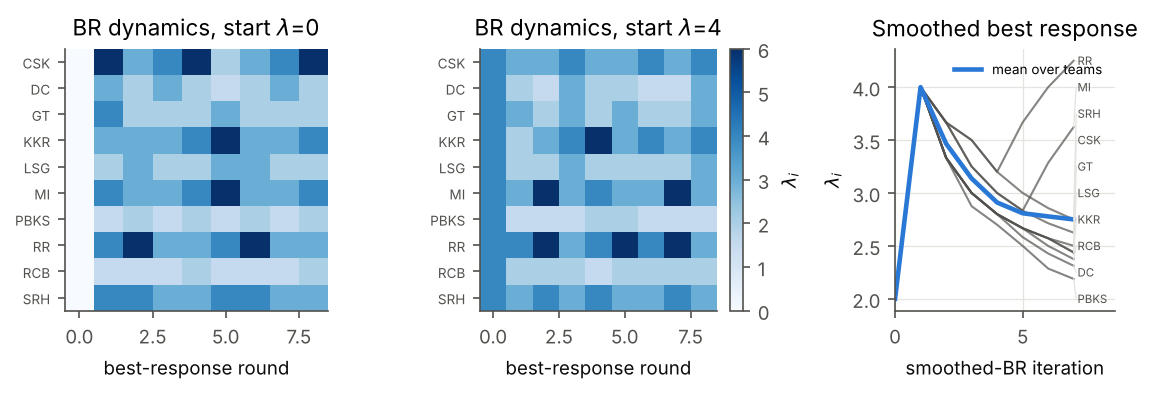
\includegraphics[width=0.9\linewidth]{../figures/fig_rq3.png}
\caption{RQ3. Plain best-response dynamics from $\lambda\equiv0$ and $\lambda\equiv4$ enter a 4-round cycle (rounds 1--4 repeat as 5--8). Right: smoothed best response contracts towards $\lambda\in[2.2,4.3]$.}
\label{fig:rq3}
\end{figure}
Plain BR dynamics do \emph{not} converge (Fig.~\ref{fig:rq3}). From both starting profiles they enter a cycle of period four within a band $\lambda_i\in[1.5,6]$, i.e.\ every team bids between $1/7$ and $2/5$ of its estimate. The large-purse teams PBKS and RCB consistently shade least. The existence result of~\citet{conitzer2022} covers static markets; here spend depends on others' multipliers through the lot order. Smoothed BR contracts (largest step 0.34 by iteration 7) but leaves $\epsilon=17\%$ of utility. The time-average of the BR cycle is closer to an equilibrium ($\epsilon=\rupee10.1\crore$, 14\% of that team's utility) and is used as $\lambda^\ast=(3.75,2.12,2.25,4.0,2.5,4.0,1.75,4.0,1.62,3.5)$ for (CSK, DC, GT, KKR, LSG, MI, PBKS, RR, RCB, SRH). Pacing is collectively valuable: league utility is $1{,}015\pm24$\crore{} at $\lambda^\ast$ vs.\ $320\pm21$ when all bid naively. At a common $\lambda=2$, teams spend 85\% of their purses.

\subsection{Validation against the real 2025 auction (feedback 1)}\label{sec:r-valid}
\begin{table}[t]
\centering\small
\caption{Simulated vs.\ real 2025 auction (100 seeds, value prior fitted on 2022 unless noted; set-wise order). KS: Kolmogorov--Smirnov distance of sold log prices; $\rho$: Spearman between a player's mean simulated and real price (players sold in reality); AUC: does sale frequency predict being sold; role MAD: mean absolute error of the team $\times$ role purchase counts.}
\label{tab:valid}
\resizebox{\linewidth}{!}{\begin{tabular}{@{}lrrrrrrrrr@{}}\toprule
Opponent model & sold & median & mean & max & spend & KS & $\rho$ & AUC & role MAD\\\midrule
Naive & 134 & 0.47 & 4.77 & 57.2 & 641 & 0.23 & 0.59 & 0.67 & 2.38\\
Eq.~(5) equilibrium & 136 & 1.56 & 4.70 & 53.6 & 639 & 0.14 & 0.69 & 0.71 & 2.28\\
Pacing equilibrium $\lambda^*$ & 196 & 0.99 & 2.30 & 31.5 & 450 & 0.13 & 0.74 & 0.73 & 2.70\\
Need-aware pacing $\lambda^*$ & 199 & 0.75 & 2.08 & 31.7 & 414 & 0.16 & 0.77 & 0.75 & 2.01\\
\midrule Real 2025 & 182 & 1.50 & 3.51 & 27.0 & 639 & -- & -- & -- & --\\
Pacing eq., prior fit 2018--24 & 199 & 0.88 & 2.06 & 29.5 & 410 & 0.15 & 0.74 & 0.71 & 2.90\\
Pacing eq., prior fit 2025 (in-sample) & 202 & 0.84 & 1.72 & 23.1 & 348 & 0.20 & 0.77 & 0.75 & 2.80\\
\bottomrule\end{tabular}
}
\end{table}
\begin{figure}[t]
\centering
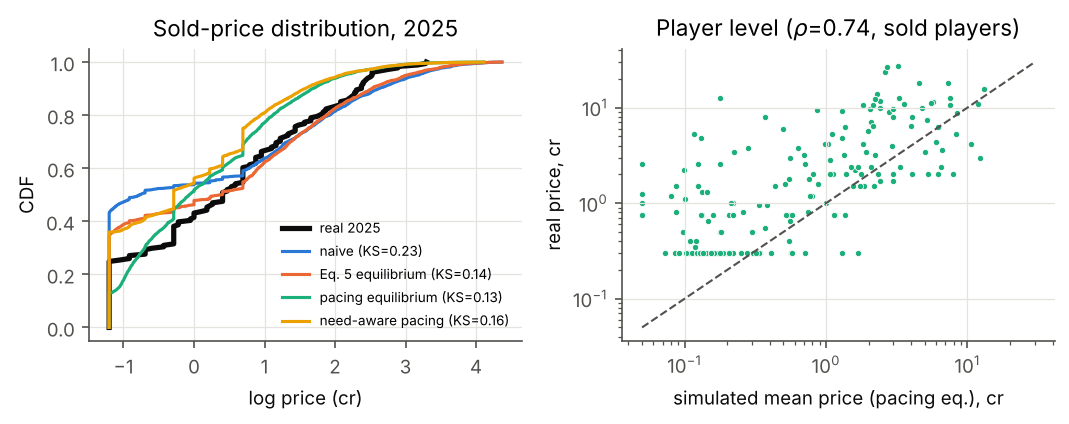
\includegraphics[width=0.9\linewidth]{../figures/fig_validation.png}
\caption{Validation. Left: CDF of sold log prices, simulated vs.\ real 2025. Right: player-level mean simulated price (pacing equilibrium) vs.\ real price.}
\label{fig:valid}
\end{figure}
No parameter in Table~\ref{tab:valid} was tuned on 2025. The pacing equilibrium, computed entirely inside the simulator, reproduces the real price distribution best (KS $0.13$ vs.\ $0.23$ for naive bidding) and caps the top price near the real \rupee27\crore{} (mean maximum 31.5\crore{} vs.\ 57\crore{} for naive bidders). It also ranks players well ($\rho=0.74$). Its main miss is the price \emph{level}: simulated teams spend about 450\crore{} against the real 639\crore{} (Fig.~\ref{fig:valid}, right, points above the diagonal). Real franchises shade less than our equilibrium predicts, plausibly because unspent purse has little value to them ($\alpha<1$). Two observations bear on the review's feedback. First, the in-sample 2025 scale fits the price distribution \emph{worse} (KS 0.20) than the 2022 scale, so the old non-independent check would not have produced a better simulator. Second, team-specific (need-aware) values give the best player-level ranking ($\rho=0.77$, AUC $0.75$) and reproduce \emph{who bought which roles} markedly better (role MAD 2.01 vs.\ 2.70).

\subsection{RQ2 and RQ4: budget-aware vs.\ myopic and learned bidding}\label{sec:r-rq2}
\begin{table}[t]
\centering\small
\caption{Mean utility (\crore) of a focal team against nine opponents playing $\lambda^\ast$ (100 seeds; 95\% CI $\approx\pm2$--$12$, Fig.~\ref{fig:rq2}). RR/DC/PBKS have real purses of 41/73/110.5\crore; DC is also run with purses scaled $\times0.5$ and $\times2$ for every team. Last column: utility over the hindsight optimum~\eqref{eq:ilp}, averaged over configurations.}
\label{tab:rq2}
\resizebox{0.54\linewidth}{!}{\begin{tabular}{@{}lrrrrrr@{}}\toprule
Focal agent & RR & DC & PBKS & DC $\times0.5$ & DC $\times2$ & $U/\mathrm{OPT}$\\\midrule
Naive $\hat v$ & 43.8 & 82.7 & 122.0 & 46.8 & 115.5 & 0.26\\
Shade 0.85 & 45.6 & 84.8 & 127.8 & 47.7 & 121.0 & 0.27\\
Eq.~(5) & 48.0 & 90.8 & 136.9 & 50.5 & 130.4 & 0.30\\
Pacing $\lambda^*_i$ & 76.4 & 113.1 & 143.9 & 86.6 & 115.1 & 0.36\\
Dual pacing (9) & 48.8 & 93.8 & 143.1 & 50.9 & 134.8 & 0.30\\
Q-learning & 42.2 & 88.7 & 134.5 & 55.9 & 137.5 & 0.29\\
DP (6)--(7) & 100.6 & 149.9 & 197.0 & 207.0 & \textbf{192.1} & 0.59\\
DP + Eq.~(5) & \textbf{120.3} & \textbf{153.9} & \textbf{203.9} & \textbf{216.4} & 186.7 & 0.63\\
\bottomrule\end{tabular}
}\hfill\resizebox{0.43\linewidth}{!}{\begin{tabular}{@{}lrrrrr@{}}\toprule
Share of DP gain over naive & RR & DC & PBKS & DC $\times0.5$ & DC $\times2$\\\midrule
Pacing $\lambda^*_i$ & 57\% & 45\% & 29\% & 25\% & -1\%\\
Dual pacing (9) & 9\% & 16\% & 28\% & 3\% & 25\%\\
Q-learning & -3\% & 9\% & 17\% & 6\% & 29\%\\
DP + Eq.~(5) & 135\% & 106\% & 109\% & 106\% & 93\%\\
\bottomrule\end{tabular}
}
\end{table}
\textbf{RQ2.} The DP bidder dominates myopic bidding everywhere (Table~\ref{tab:rq2}). It earns $2.3\times$ the naive utility for the tight-purse RR, $1.8\times$ for DC, $1.6\times$ for PBKS, $4.4\times$ when every purse is halved, and $1.7\times$ when every purse is doubled. The gain is largest when the purse binds, as hypothesised. It comes from spending less on the first stars and more on the many cheap but valuable players that the paced market leaves behind (DC: 20.4 players for \rupee64.5\crore{} vs.\ 16.6 for \rupee72.3\crore{} when naive). Fixed pacing at $\lambda^\ast_i$ recovers 25--57\% of the DP's gain under real or tight purses but nothing when purses are doubled. A single multiplier cannot tell early stars from late bargains. Combining the DP with the curse correction (DP+Eq.~(5)) is best in four of five settings (RR: $+20\crore$); RQ1 and RQ2 are complementary. Proposition~\ref{prop:threshold} holds numerically: on 300 random states, brute-force search over drop-out prices against the pilot samples finds the closed-form $a^\ast_t$ optimal in 98\% of states, with a largest loss of \rupee0.005\crore. The DP is insensitive to the purse grid (utility 149.0, 149.6, 150.9, 148.2 for grids 0.1, 0.25, 0.5, 1.0\crore; $\pm8$). Its own forecast (200.6 for DC) is optimistic by 25\%, because rival behaviour responds to the focal team's purchases.

\textbf{RQ4.} Without an opponent model, little of the DP's advantage survives. Dual pacing~\eqref{eq:dual} recovers 3--28\%; its multiplier reacts to spend that is front-loaded in the set-wise order, so it under-shades early stars (Fig.~\ref{fig:dual}, Appendix). Q-learning trained for 1{,}500 auctions recovers $-3$ to 29\%. Its learning curve (DC, Fig.~\ref{fig:rl}, Appendix) rises from 62 to about 100\crore{} within 1{,}500 episodes, is unstable (it drops to 44 at 3{,}000 episodes), and ends at 115 after 6{,}000 episodes. That is the level of the pacing equilibrium (113) and well below the DP (150), so more training does not close the gap. The DP's advantage is therefore mostly the value of \emph{knowing how rivals bid on each lot}.

\subsection{Team-specific values (feedback 2)}\label{sec:r-xi}
\begin{figure}[t]
\centering
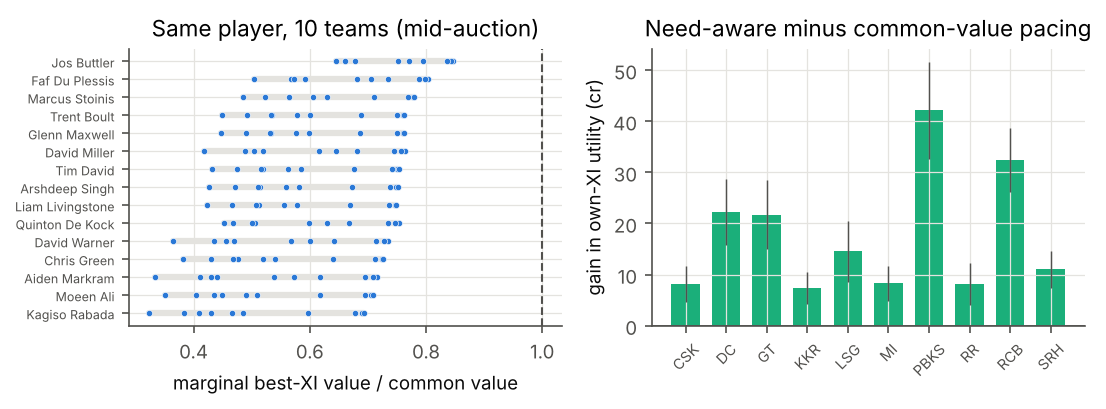
\includegraphics[width=0.8\linewidth]{../figures/fig_team_specific.png}
\caption{Left: marginal best-XI value of the top players to each of the ten teams halfway through the auction, relative to their common value (20 seeds). Right: gain in own-XI utility from need-aware rather than common-value pacing, focal team vs.\ nine $\lambda^\ast$ opponents (60 seeds, 95\% CI).}
\label{fig:xi}
\end{figure}
At the start of the auction every squad has fewer than 11 players, so any purchase walks into the XI and values coincide. Halfway through they do not (Fig.~\ref{fig:xi}): the same top-40 player is worth on average 22\% of his common value to the team that needs him least and 76\% to the team that needs him most (cross-team coefficient of variation 0.41). Teams that bid on their own needs gain in own-XI utility in \emph{all ten} cases, from $+7\crore$ (KKR) to $+42\crore$ (PBKS), mean $+17.6\crore$. If every team is need-aware, league utility rises from $656\pm33$ to $724\pm34$. Part of the gain is a budget effect: diminishing marginal value makes need-aware agents shade later purchases, and they also do better under the common-value utility ($+20.8\crore$). Together with the improved role allocation in Table~\ref{tab:valid}, this supports the review's suggestion: a player is not worth the same to every team, and modelling this helps both prediction and decisions.

\subsection{Sale order and a real-data test of the curse}\label{sec:r-order}

Prices decline as purses drain, the ``afternoon effect''~\citep{ashenfelter1989}. In random order price/value falls from 0.39 in the first decile to 0.20 in the last. In the set-wise order it falls within the capped block (0.37 to 0.22), jumps to 0.34 when the uncapped sets begin, and falls again (Fig.~\ref{fig:order}, Appendix). This decline is what the DP exploits. On real data (Fig.~\ref{fig:order}, right), the sold players under-performed our pre-auction prediction by $1.36\pm0.52$ runs/match in the 2025 season. The slope of that shortfall on the price premium teams paid over the public model is $0.87$ (95\% CI $[-0.20,1.95]$), far below the slope of 23 that the premium would imply if it reflected better on-field impact. Premiums were not repaid on the field, which is consistent with a winner's curse. It could also reflect value our batting/bowling metric does not capture (captaincy, fielding, marketing).

% ===============================================================
\section{Discussion and Limitations}
\label{sec:discussion}
Two lessons stand out: (1) when budgets bind, curse diagnostics based on overpayment are misleading and belief bias plus utility must be reported, and (2) the value of budget-aware planning comes mostly from anticipating where in the auction prices will be low. \textbf{Limitations.} The money scale is fitted on sold players only, which overstates the value of marginal players. Public data contain no bidding sequences, so rival behaviour is modelled (pacing equilibrium), and simulated prices are about 30\% lower than real ones. The 2025 lot order is reconstructed. Right-to-match cards are excluded. The DP ignores overseas counts in its state (the simulator enforces them) and conditions on $\hat v$ rather than on the rivals' drop-outs. The BR analysis uses a 10-point grid and 12--20 seeds. Roles and nationality were imputed for 281 and 264 low-profile lots.

% ===============================================================
\section{Contributions}
\label{sec:contrib}
All members contributed to discussions, debugging and writing; Table~\ref{tab:contrib} lists primary responsibilities. The code is at \url{\repourl}; \texttt{run\_all.sh} regenerates every number, table and figure. 
\begin{table}[h]
\centering\footnotesize
\caption{Work packages, owners and status.}
\label{tab:contrib}
\begin{tabularx}{\linewidth}{@{}lXl@{}}
\toprule
Member & Assigned tasks & Status\\
\midrule
Harshvarshan Masalge & Data pipeline: Cricsheet parsing, name matching and alias table, auction and retention data; repository, README and reproducibility script; out-of-sample validation against 2025 (Sec.~\ref{sec:r-valid}). & Completed\\
Advait Andhale & Equilibrium bid~\eqref{eq:beta} and its single-lot verification; winner's-curse experiments and the tight-budget analysis (RQ1, feedback 3; Sec.~\ref{sec:r-curse}); sale-order experiment. & Completed\\
Onkar Gaikwad & Constrained MDP, proof and numerical check of Prop.~\ref{prop:threshold}, DP bidder; pacing equilibrium and BR dynamics; dual pacing and Q-learning agents (RQ2--RQ4). & Completed\\
Shreyash Pandit & Empirical-Bayes value model and money scale fitted on 2022 (feedback 1); best-XI team-specific values and need-aware agent (feedback 2); hindsight ILP; real-data ex-post test. & Completed\\
\bottomrule
\end{tabularx}
\end{table}

\bibliographystyle{unsrtnat}
\bibliography{references}

\clearpage
\appendix
\section{Supplementary material}
\begin{table}[h]
\centering\small
\caption{Pre-auction state of the 2025 mega auction used by the simulator (purse in \crore, retained players, of which overseas).}
\label{tab:teams}
\begin{tabularx}{\linewidth}{@{}lrrrX@{}}\toprule
Team & purse & $m^0$ & $q^0$ & retained players\\\midrule
CSK & 55.0 & 5 & 1 & \footnotesize Ruturaj Gaikwad, Ravindra Jadeja, Matheesha Pathirana, Shivam Dube, MS Dhoni\\
DC & 73.0 & 4 & 1 & \footnotesize Axar Patel, Kuldeep Yadav, Tristan Stubbs, Abishek Porel\\
GT & 69.0 & 5 & 1 & \footnotesize Rashid Khan, Shubman Gill, Sai Sudharsan, Rahul Tewatia, Shahrukh Khan\\
KKR & 51.0 & 6 & 2 & \footnotesize Rinku Singh, Varun Chakaravarthy, Sunil Narine, Andre Russell, Harshit Rana, Ramandeep Singh\\
LSG & 69.0 & 5 & 1 & \footnotesize Nicholas Pooran, Ravi Bishnoi, Mayank Yadav, Mohsin Khan, Ayush Badoni\\
MI & 45.0 & 5 & 0 & \footnotesize Jasprit Bumrah, Suryakumar Yadav, Hardik Pandya, Rohit Sharma, Tilak Varma\\
PBKS & 110.5 & 2 & 0 & \footnotesize Shashank Singh, Prabhsimran Singh\\
RR & 41.0 & 6 & 1 & \footnotesize Sanju Samson, Yashasvi Jaiswal, Riyan Parag, Dhruv Jurel, Shimron Hetmyer, Sandeep Sharma\\
RCB & 83.0 & 3 & 0 & \footnotesize Virat Kohli, Rajat Patidar, Yash Dayal\\
SRH & 45.0 & 5 & 3 & \footnotesize Heinrich Klaasen, Pat Cummins, Abhishek Sharma, Travis Head, Nitish Kumar Reddy\\
\bottomrule\end{tabularx}

\end{table}
\begin{figure}[h]
\centering
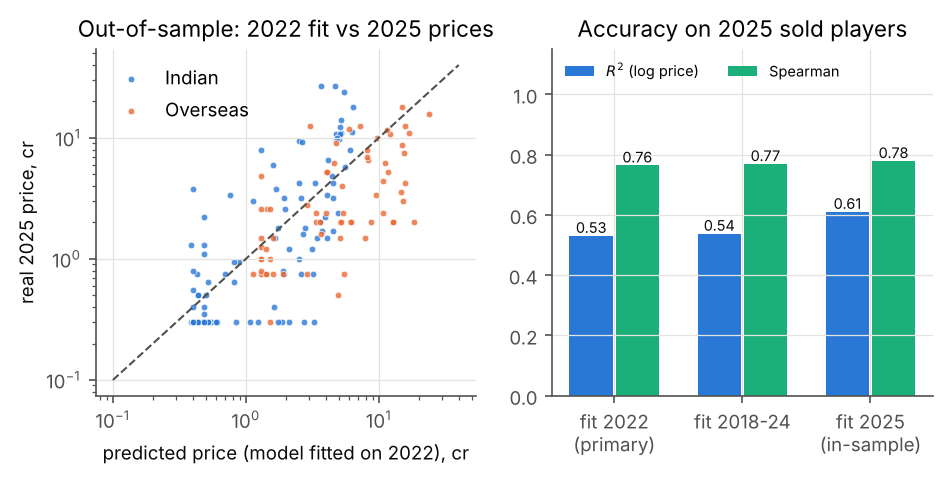
\includegraphics[width=\linewidth]{../figures/fig_money_scale.png}
\caption{Money scale fitted on 2022 vs.\ real 2025 prices (left) and accuracy of the three fits on 2025 (right).}
\label{fig:scale}
\end{figure}
\begin{figure}[h]
\centering
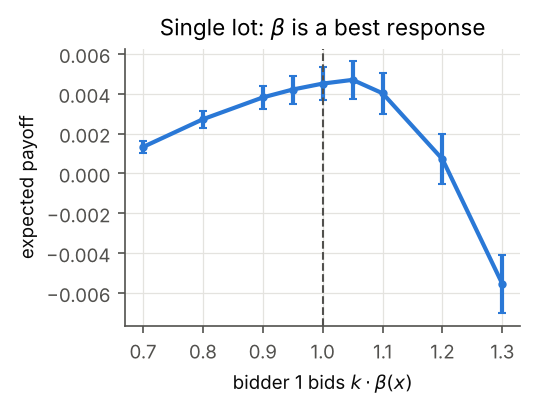
\includegraphics[width=0.42\linewidth]{../figures/fig_beta_check.png}\hfill
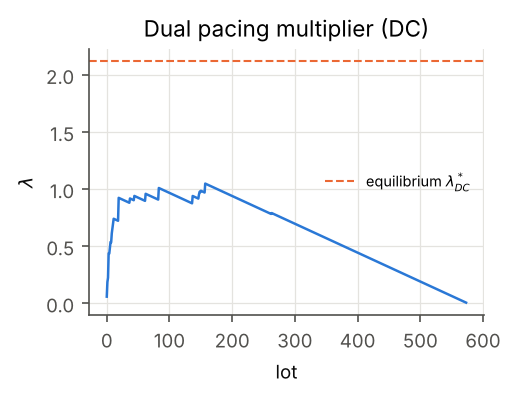
\includegraphics[width=0.42\linewidth]{../figures/fig_dual_trace.png}
\caption{Left: single-lot check of Eq.~\eqref{eq:beta}; bidder 1 scales its bid by $k$ against nine $\beta$-bidders (60{,}000 draws, 95\% CI). Right: dual-pacing multiplier over one auction (DC) vs.\ the equilibrium $\lambda^\ast_{\rm DC}$.}
\label{fig:beta}\label{fig:dual}
\end{figure}
\begin{figure}[h]
\centering
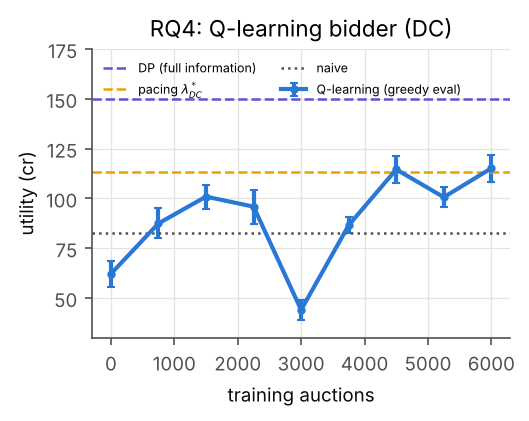
\includegraphics[width=0.48\linewidth]{../figures/fig_rl_curve.png}\hfill
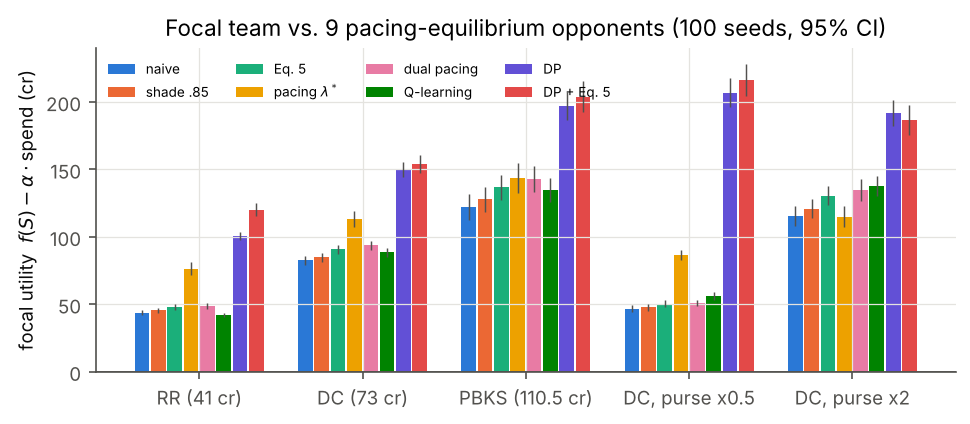
\includegraphics[width=0.5\linewidth]{../figures/fig_rq2_rq4.png}
\caption{Left: Q-learning learning curve for DC (30 evaluation seeds per point) with the pacing-equilibrium and DP levels. Right: utilities of Table~\ref{tab:rq2} with 95\% CIs.}
\label{fig:rl}\label{fig:rq2}
\end{figure}
\begin{figure}[h]
\centering
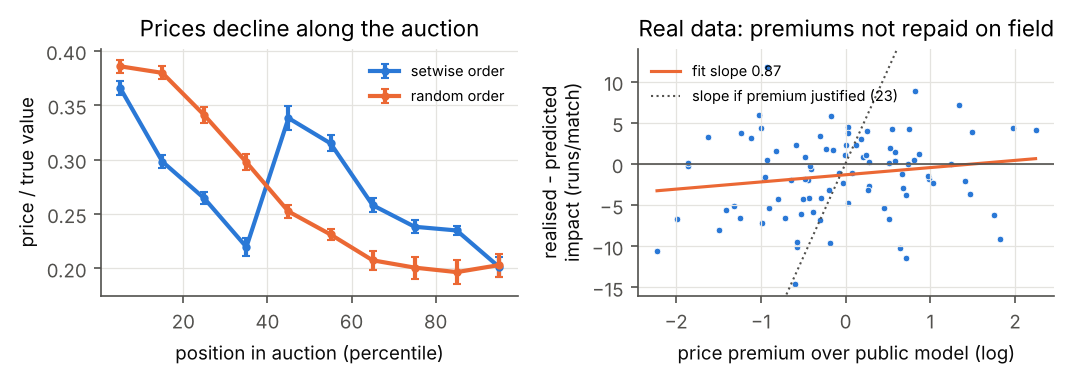
\includegraphics[width=\linewidth]{../figures/fig_order_expost.png}
\caption{Left: price/value by position in the auction (pacing equilibrium, 60 seeds). Right: real 2025 data. A player's price premium over our public pre-auction model vs.\ his realised minus predicted impact in the 2025 season ($n=89$ sold players with $\ge5$ matches).}
\label{fig:order}
\end{figure}
\end{document}
